\subsection{QuizziPedia::Back-End::App::Controllers::Errors}
\subsubsection{Informazioni generali}
\label{QuizziPedia::Back-End::App::Controllers::Errors}
\begin{figure}[ht]
	\centering
	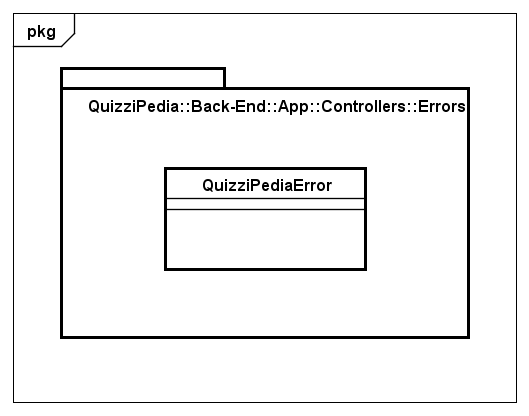
\includegraphics[scale=0.45]{UML/Package/QuizziPedia_Back-End_App_Controllers_Errors.png}
	\caption{QuizziPedia::Back-End::App::Controllers::Errors}
\end{figure}
\FloatBarrier
	\begin{itemize}
		\item \textbf{Descrizione} \\
		Package contenente i controllers per la gestione degli errori specifici.
		\item \textbf{Padre}: \texttt{Controllers}
	\end{itemize}
\subsubsection{Classi}
\paragraph{QuizziPedia::Back-End::App::Controllers::Errors::QuizziPediaError}
	\begin{itemize}
		\item \textbf{Descrizione} \\
		Classe che contiene gli errori. Esegue la costruzione del messaggio d'errore specifico per i moduli di \texttt{QuizziPedia::Back-End::App}.
		\item \textbf{Utilizzo} \\
		Viene utilizzato da \texttt{ErrorsHandler} quando di verifica un errore specifico relativo alle classi di \texttt{QuizziPedia::Back-End::App}
		\item \textbf{Relazioni con altre classi}:
			 \begin{itemize}
			 	\item \textit{IN} \texttt{ErrorsHandler} \\
			 	Classe middleware\ped{G} per la gestione delgi errori. Ritorna al client un oggetto di tipo \texttt{Response} con stato HTTP\ped{G} 500 e descrizione dell'errore in formato JSON\ped{G}. E' un componente \texttt{ConcreteHandler} del desing pattern \textit{Chain of responsability\ped{G}}.
			 \end{itemize}
		\item \textbf{Attributi}:
			 \begin{itemize}
			 	\item 
			 \end{itemize}
		\item \textbf{Metodi}:
			\begin{itemize}
				\item 
			\end{itemize}
	\end{itemize}